%%%%%%%%%%%%%%%%%%%%%%%%%%%%%%%%%%%%%%%%%%%%%%%%%%%%%%%%%%%%%%%%%%%%%%%%
% RevTeX 4.1 LaTeX
% Kevin C. Young
% Scalable & Secure Systems Research (08961)
% Thu Mar  5 15:29:19 PST 2015
%%%%%%%%%%%%%%%%%%%%%%%%%%%%%%%%%%%%%%%%%%%%%%%%%%%%%%%%%%%%%%%%%%%%%%%%

\documentclass[aps,nofootinbib,pra,notitlepage,twocolumn]{revtex4-1}
\usepackage{amsfonts,amsmath,amssymb,amsthm}
\usepackage{array,bm,color}
\usepackage{epsfig,graphicx,nomencl,revsymb4-1,upgreek,url}
\usepackage{hyperref}
\usepackage{algorithm}
\usepackage{algpseudocode}
\usepackage{graphicx}
\graphicspath{{./figures/}}
\hypersetup{colorlinks=true, pdfauthor=Kevin C. Young, pdftitle=Decorrelating Errors}
\newcommand{\tr}{{\rm Tr\thinspace}}
\newcommand{\bra}[1]{\ensuremath{\left\langle{#1}\right\vert}}
\newcommand{\ket}[1]{\ensuremath{\left\vert{#1}\right\rangle}}
\newcommand{\braket}[2]{\left\langle #1 | #2 \right\rangle}
\newcommand{\ketbra}[2]{\left| #1 \right\rangle\!\!\!\,\left\langle #2 \right|}
\newcommand{\abs}[1]{\left\vert #1 \right\vert}
\newcommand{\expect}[1]{\ensuremath{\left\langle{#1}\right\rangle}}
\newcommand{\timeorder}{\ensuremath{\underset{\leftarrow}{\mathcal{T}}}}
\newcommand{\ident}{{\mathbb1}}
\newcommand{\order}[1]{\mathcal{O}\left( #1 \right)}
\newcommand{\diag}[1]{\mathrm{diag}\{#1\}}
\newcommand{\trans}[1]{#1^\mathsf{T}}
\newcommand{\T}{\mathsf{T}}
\newcommand{\erf}[1]{Eq.~(\ref{#1})}
\newcommand{\needcite}{{\color{blue}\textsuperscript{[citation needed]}}}
\newcommand{\note}[1]{{\color{red}[#1]}}
\newcommand{\kcy}[1]{{\color{red}[#1]_{\rm{KCY}}}}
\newcommand{\amp}[1]{{\color{red}[#1]_{\rm{AMP}}}}
\setlength{\jot}{10pt}
\newtheorem{thm}{Theorem}[section]
\newtheorem{lem}[thm]{Lemma}
\usepackage{lipsum}

\begin{document}

\section{Numerics}
In this section, we numerically assess the performance of 0RBCs and 1RBCs. In particular we consider two tunable qubits, coupled by a resonant exchange interaction, inspired by systems like that in \cite{https://arxiv.org/pdf/1604.03076.pdf}.  For the one-qubit case then, we generate a 1RBC for $RX(\frac{\pi}{2})$ and $RY(\frac{\pi}{2})$. Our control Hamiltonian is given as:
\begin{equation}\label{eq:1Qham}
  H(\delta, \epsilon, t) = \epsilon\sigma_z + (1 + \delta)(c_x(t)\sigma_x + c_y(t)\sigma_y)
\end{equation}
where $\epsilon$ corresponds to fluctuations in qubit frequency given by noise on the flux line, and $\delta$ corresponds to fluctuations in the drive amplitude given by noise on the qubit RF drive line. Using the MOSEK solver in cvxpy, and imposing the sparsity constraint in \cite{SPARTSITY}, we generated weights for 0RBCs and 1RBCs, containing just ten controls. The controls were generated via the GRAPE algorithm described in Section \ref{GRAPE SECTION}, assuming Gaussian Noise with mean 0, and standard deviation $.001$. We gave GRAPE a total evolution time of $\pi$, compared with the required $\frac{pi}{2}$ time for the shortest path. We discretized the evolution into 25 steps, and generated 200 controls for the convex solver to choose from. The resutls are shown in \ref{FIGURE1}  and\ref{FIGURE2}. In both cases it can be seen that near the origin the 0RBC and 1RBC outperform the constituent controls by two orders of magnitude in diamond norm, and away from the origin the 0RBC can be seen to increase in diamond norm more quickly than the 1RBC. 

\begin{figure}[htb]
  \centering
  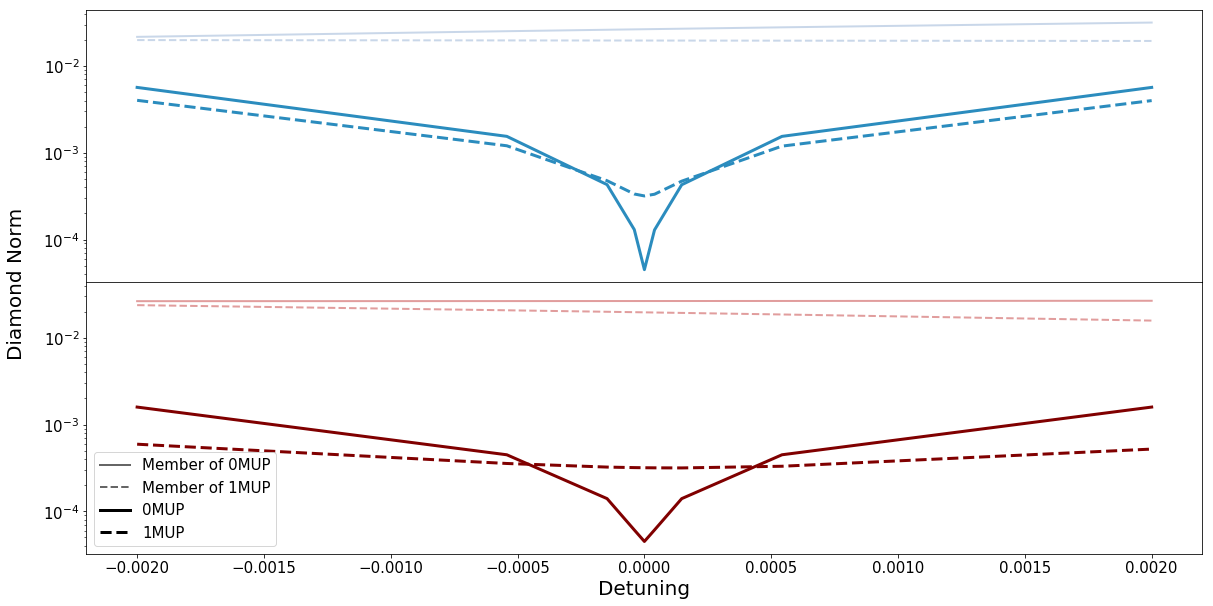
\includegraphics[scale=.2]{figures/SQRTX}

\caption{0RBC and 1RBC performance for $RX(\frac{\pi}{2})$, as compared to each other, and members of the control families. At the origin the RBCs can be see to outperform members of the family by two orders of magnitude in diamond norm. Away from the origin the 1RBC can be seen to be flatter than the 0RBC, outperforming at 1\% error.}
\end{figure}
\begin{figure}[htb]
  \centering
  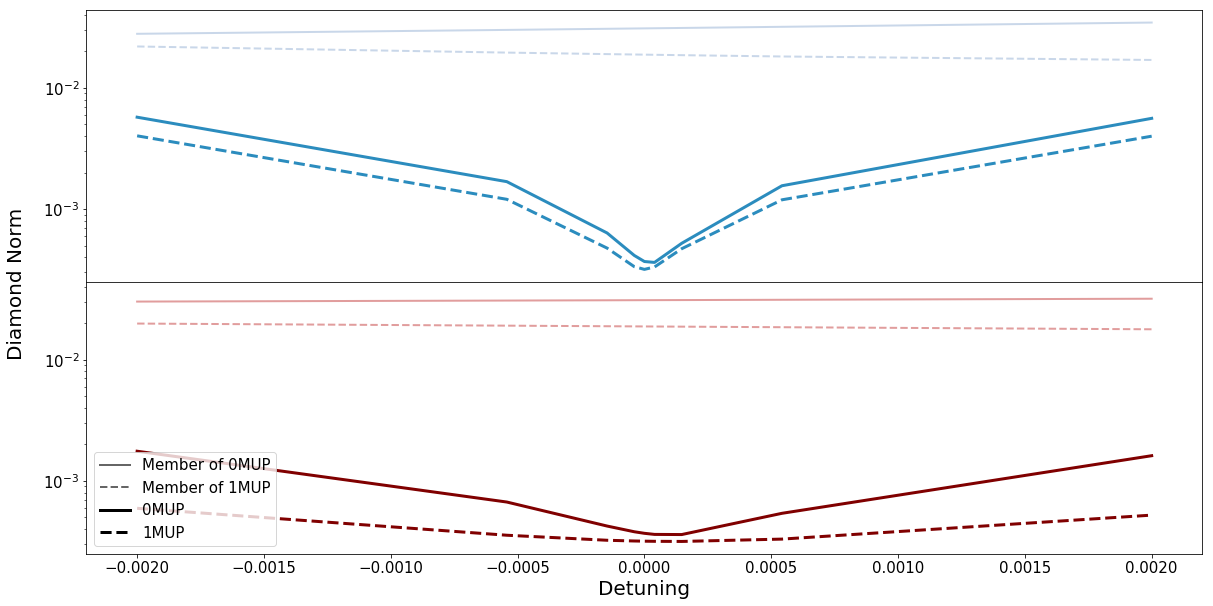
\includegraphics[scale=.2]{figures/SQRTY}
\caption{0RBC and 1RBC performance for $RX(\frac{\pi}{2})$, as compared to each other, and members of the control families. At the origin the RBCs can be see to outperform members of the family by two orders of magnitude in diamond norm. Away from the origin the 1RBC can be seen to be flatter than the 0RBC, outperforming at .5\% error.}
\end{figure}

For the two qubit example we extend our one qubit model to include a resonant exchange interaction. Our control Hamiltonian is given as:
\begin{equation} \label{eq:2Qham}
\begin{split}
H(\vec{\epsilon}, \vec{\delta}, t) = &\sum_{j=1}^2(\epsilon_j\sigma_z^j + (1 + \delta_j)(c_x^jx(t)\sigma_x^j + c_y^j(t)\sigma_y^j)) \\
&+ k(XX + YY)
\end{split}
\end{equation}

There were several difficulties in considering this particular Hamiltonian, and for more interesting results one might consider a Hamiltonian with a control on the interaction -- such as that of a tunable coupler used in \ref{https://arxiv.org/pdf/1402.7367.pdf}. With that Hamiltonian it is non-trial to construct control solutions that are insensitive to detuning errors on either qubit, since such sequences also tend to decouple the entangling interaction.

Moreover, when attemping to construct control solutions for \ref{eq:2Qham} GRAPE failed to find anything non-trivial. Therefore for this example we constructed analytic bangbang \ref{BANGBANG} sequences that flip both qubits at different times in the sequence to affect a decoupling of detuning errors, while remaining invariant to the eigenspaces of the interaction term. To give the control family a variety of different errors, we added on uniformly distributed errors to each $\pi$ pulse, between $-.25$\% and $.25$\%. A plot of typical control amplitude sequence is given in Figure  \ref{FIGURE}.

Using the same piecewise constant control solution as in the one qubit case, we considered 100 steps, with a total evolution time of $\frac{5\pi}{2}$, the time required for the $XX + YY$ interaction to generate an iSWAP gate in the absence of any other controls. In this case, we treated the $RX(\pi)$, $RX(-\pi)$, $RY(\pi)$ and $RY(-\pi)$ pulses used to decouple the tuning errors as taking only one time step, to avoid significant errors arising from mixing the eigenspaces of the interaction term. In practice this could be accomplished instead by turning off the resonance, performing the $\pi$ pulse, and turning the interaction back on. The particular collection of bang-bang sequences considered were all combinations of of simultaneous $\pi$ pulses activated at multiples of $8$ steps from the first time step, and the same multiple of $8$ steps prior to the last time step. This resulted in a control family of 1024 controls. We did not apply the sparsity constraint to the solutions, however over 100 of the controls have less than $.5$\% of support, so it is feasible that the sparsity constraint could be successfully applied. 

The $0RBC$ succesfully finds weights that minimize the 0th order term in the error Hamiltonian to zero within numerical precision, but with nonzero first derivative. Given the 1RBC minimization problem, the solver can also successfully supress the first derivative, while keeping the zeroth order term 0. At the origin, both RBCs can be seen to perform equally well, and better than members of the control family. Away from the origin both RBCs can be seen to perform over half an order of magnitude better in diamond norm than members of the control family, with the 1RBC degrading in quality more slowl than the 0RBC.

There is much more work that can be done investigating other Hamiltonians, for other kinds of noise, and more interesting compositive pulse sequences that might be system dependent. In addition, imposing the $\ell_1$ constraint has the potential to increase performance of $RBC$s when the members of the control family have varied performance (constrasted with the scenario given in Campbell's paper \ref{Campbell} where all controls are assumed to have error bounded by $\epsilon$.) Investigating the trade off between controls with slightly worse error but more interesting derivative may provide more favorable performance increases.

Finally, much of the numerical work here was limited by the same simplicity that makes the GRAPE algorithm useful. Future work could modify the derivative in the GRAPE algorithm to include derivative information to in addition to finding controls with bounded error, GRAPE finds controls with not only bounded derivative, but also derivatives that are wrong in a way that can cancel out the derivatives of other controls in the RBC. These results demonstrate numerically that RBCs are feasible and tractable, and provide an algorithmic way to compute optimal weights for minimizing sensitive to drift.


\end{document}